\chapter{Three-Loop Breakdown}

One convenient way of understanding how the GPGPU works is through
looking at its three main scheduling loops that run within every SM.
This is the approach taken by \cite{aamodt2018general}.
The textbook builds the architecture up, covering one scheduler at a time.

This section will use the three approximations introduced in the textbook but
leave the treatment of warp divergence for last. The reader is encouraged to
refer to the textbook for more details.

\section{One-Loop Approximation}

\begin{figure}[h]
    \centering
    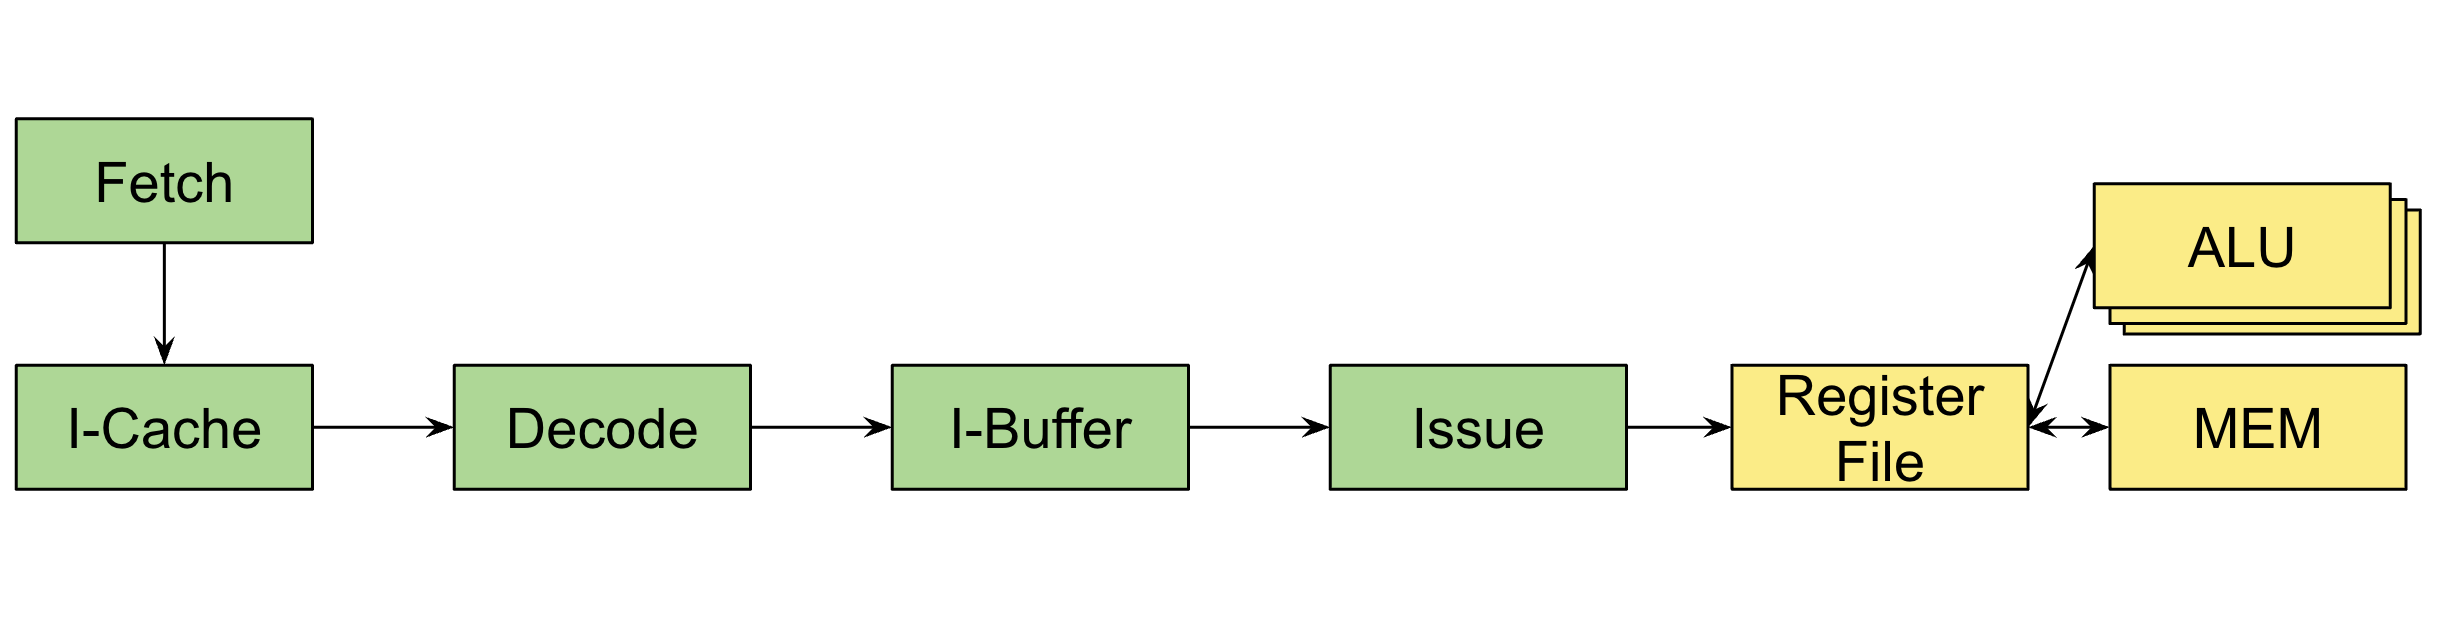
\includegraphics[width=0.5\textwidth]{assets/1.png}
    \caption{One-Loop Approximation diagram. }
    \label{fig:oneloop}
\end{figure}

The first loop is the scheduler that fetches instructions. 

Refer to Figure \ref{fig:oneloop} for a high level overview of the pipeline at this point.
The Fetch unit sends an instruction from the Instruction Cache (I-Cache) to
get Decoded before it gets saved to the Instruction Buffer (I-Buffer).

In this approximation, we can have one instruction in flight at a time for
a warp and we fetch instructions using the warp's program counter corresponding
to this instruction.

While the CPU issues many instructions at once to allow for latency
hiding, the GPU hides a significant amount of latency by Issuing
instructions for different warps at different cycles. Specifically, if we have
a warp that is performing a memory access that missed in cache, we can swap
to another warp whose next instruction uses an ALU, hiding the latency.

\section{Two-Loop Approximation}

\begin{figure}[h]
    \centering
    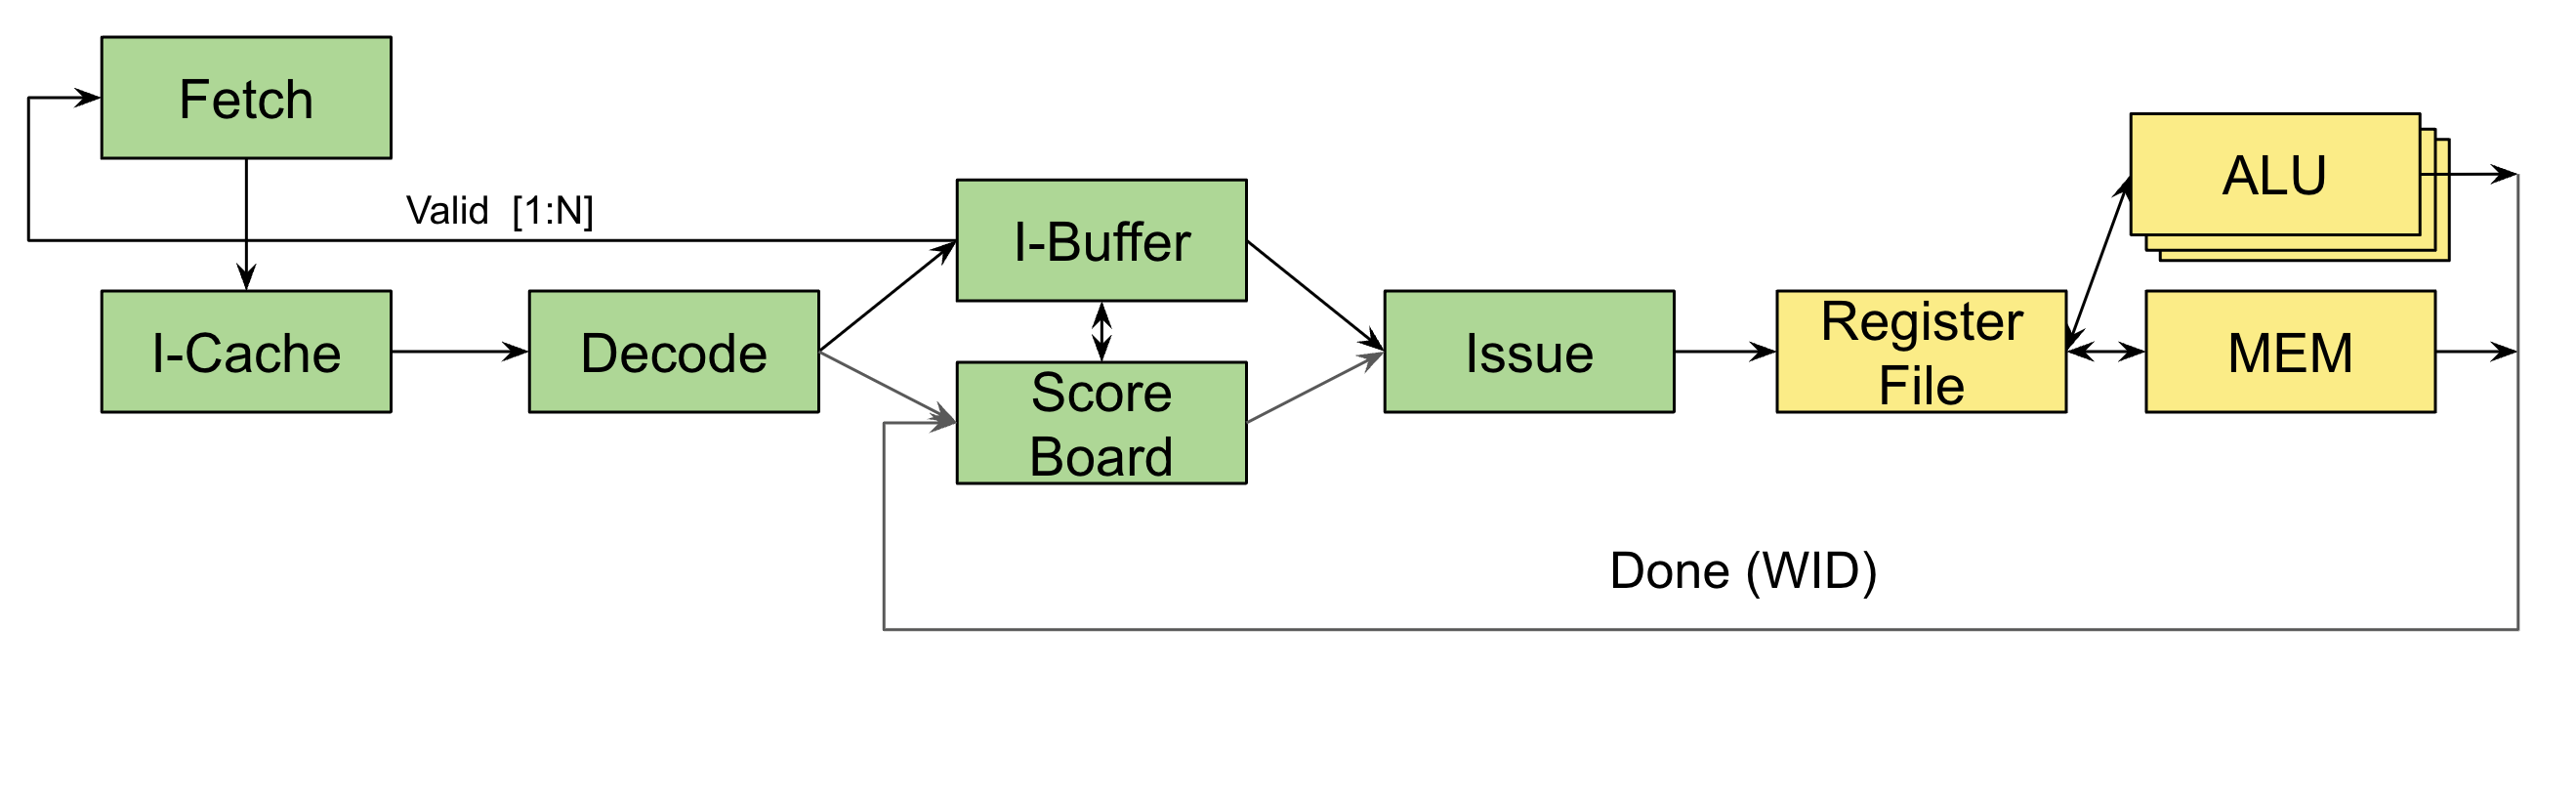
\includegraphics[width=0.5\textwidth]{assets/2.png}
    \caption{Two-Loop Approximation diagram. }
    \label{fig:twoloop}
\end{figure}

The second loop is the scheduler that chooses which instructions to issue.
Refer to Figure \ref{fig:twoloop} for a high level overview of the pipeline at this point.

In order to support swapping between warps, we need to save the values in
the registers for each warp when we context switch.
This means that our register file must have more space and be physically larger
for every warp we support.
As a result, this limits us in regards to how many warps we can allocate to an
SM. This means that past a certain point, we may need other means of hiding
latency.

Another way we can hide latency is through instruction level parallelism with multiple instructions from a warp executing at the same time.
Doing this naively can result in write-after-read hazards. As a result, we need 
some means of avoiding hazards. Since warps execute instructions in-order,
a natural solution is the scoreboard.

In in-order CPUs, scoreboards simply have a ready bit for each register.
This doesn't work for GPUs, though: we have over a thousand registers we
would need to track, occupying significant space.

One solution is the following: for each warp, keep a list of the destination
registers of all in-flight instructions. When an instruction gets added to
the I-Buffer, it can check whether its operand registers match those
in this list and save to its row in the I-Buffer a bit vector whose
bits indicate whether or not an operand is ready (set to 1) in the sense that
it will not be written to by any in-flight instructions.

In the write-back stage, the instructions update the list of registers in the scoreboard,
removing the one they write to.
They also go through all instructions in the IB for their warp and update the
ready bits for those instructions whose operand registers match its destination register.

Instructions with all bits in their bit vectors set to 1 can be scheduled in-order by the scheduler.
These then add their destination register to the scoreboard and begin execution.


\section{Three-Loop Approximation}

The third loop is the scheduler that optimizes accesses to banked register files.

A single-ported register file can be read from or written to by one operand on a given cycle.
If we want to increase the number of accesses, we can increase the number of ports, but
this requires a lot of area.

An alternative approach to enable more concurrent accesses is banking. This consists of splitting
our register file into smaller register files called banks. Each bank holds different
data and has its own read/write port. This means that each bank could be accessed in one
cycle by different operands. Accesses for operands pass through an arbitor that routes
them to the correct bank.

Registers are mapped to banks in a swizzled fashion. A naive mapping of a register to bank $r\# \ \% \ NUM\_BANKS$ would
assign registers 0 of all warps to bank 0, registers 1 to bank 1, and so on. If we try to fetch
the same register for two different warps, then, we would have to stall because we would have
two accesses to a single bank in one cycle.

Swizzling fixes this issue. It makes the warp number affect our mapping. Thus, a given register is now
assigned to bank $(r\# \ + \ W\#) \ \% \ NUM\_BANKS$.
This way, the same register on different warps maps to different banks.

\begin{figure}[h]
    \centering
    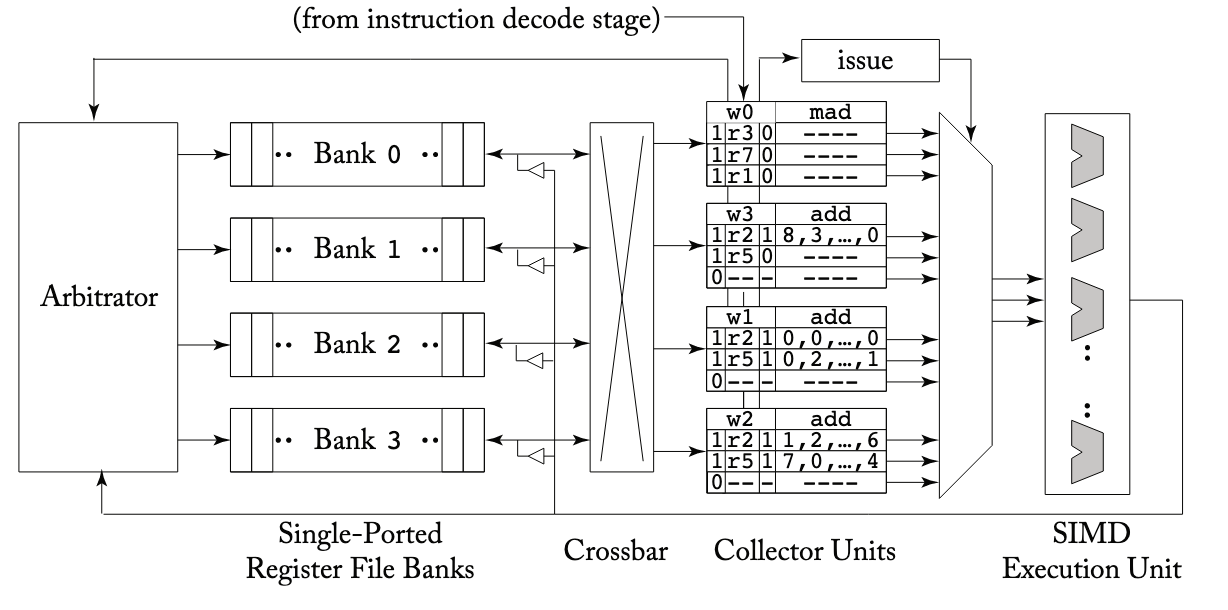
\includegraphics[width=0.5\textwidth]{assets/operand.png}
    \caption{Hardware for accessing the register file using the Operand Collector.}
    \label{fig:opcoll}
\end{figure}

To schedule operand accesses, the Operand Collector is used. This is a hardware unit that
has a slot for each instruction. These schedule register bank accesses to minimize conflicts.
Figure \ref{fig:opcoll} shows how the banked registers could be structured with an Operand Collector.

Refer to \cite{aamodt2018general} pages 35 to 40 for detailed examples that illustrate the benefits of using
the Operand Collector and bank swizzling.

\section{Warp Divergence}

This approximation has omitted handling warp divergence for the sake of simplicity.
We can have control flow in CUDA code. An example can be seen in Figure ??.

This is the same code as before, except for the fact that the size of the vector is passed
as an argument, $N$. This could be specified by a user, unlike the number of threads in a block,
which is hardcoded. We assume that $N$ is less than the number of threads in this example.

One question that might arise is what if $N$ is 16? Warps consist of 32 threads
executing in lock-step. How do we handle this?

The answer is predication: we use a mask (the SIMT Mask) to control which threads in a warp
should be active (set to 1) and inactive (set to 0) at a given point in the program's execution.

In older architectures, this masking was managed by the SIMT Stack, of which
a detailed explanation and example of can be found on
on pages 23 to 26 of \cite{aamodt2018general}. Recent GPUs use a synchronization barrier based
way of handling warp divergence and this can be found on pages 27 to 31 of \cite{aamodt2018general}.

\section{Full Architecture}


\begin{figure}[h]
    \centering
    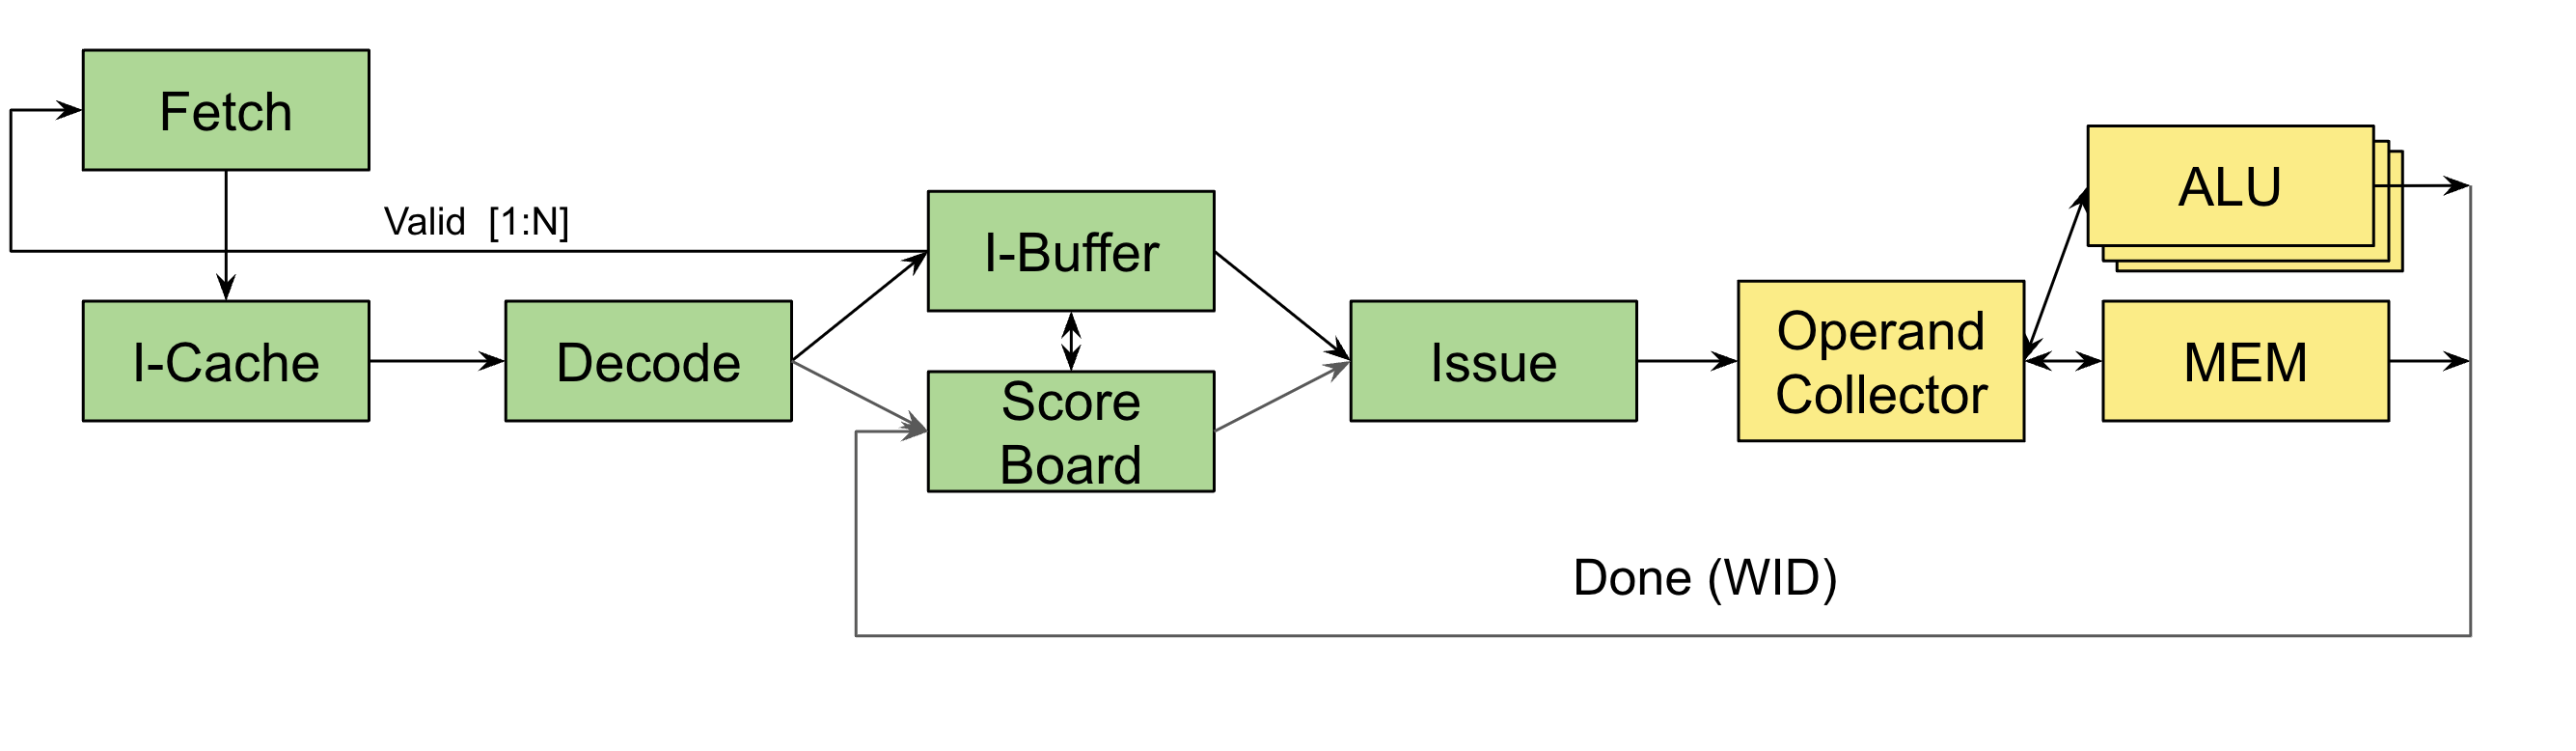
\includegraphics[width=0.5\textwidth]{assets/3.png}
    \caption{Three-Loop Approximation diagram with SIMT Stack for handling warp divergence.}
    \label{fig:warpthreeloop}
\end{figure}

With the SIMT Stack, we can assemble a diagram of the entire architecture.
This can be seen in Figure \ref{fig:warpthreeloop} 
